\documentclass[11pt]{article}
\usepackage[margin=1in]{geometry}
\usepackage{times}
\usepackage{graphicx}
\usepackage{tikz}
\usepackage{amsmath,amsfonts}
\usepackage{booktabs}
\usepackage{caption}
\usepackage{subcaption}
\usepackage{hyperref}
\usepackage{float}
\usepackage{microtype}

\usepackage[left=1in,right=1in]{geometry}
\usepackage{fancyhdr}
\usepackage{graphicx}
\usepackage{amsmath}
\usepackage{booktabs}
\usepackage[utf8]{inputenc} % allow utf-8 input
\usepackage[T1]{fontenc}    % use 8-bit T1 fonts
\usepackage{url}            % simple URL typesetting


\fancypagestyle{plain}{
  \fancyhf{}
  \fancyhead[L]{\sffamily University of Illinois Chicago}
  \fancyhead[R]{\sffamily Generative AI, Fall 2025}
%   \fancyfoot[L]{\sffamily /department of computer science}
%   \fancyfoot[R]{\sffamily\bfseries\thepage}
  \renewcommand{\headrulewidth}{0.5pt}
  \renewcommand{\headrule}{\hbox to\headwidth{%
    \leaders\hrule height \headrulewidth\hfill}}
  \renewcommand{\footrulewidth}{0pt}% No footer rule
%   \renewcommand{\footrulewidth}{0.5pt}
}
% \fancypagestyle{plain}{\homework}


\title{Design and Evaluation of a Conditional Diffusion Model for Image Generation}
\author{ChatGPT}

\date{\today}

\begin{document}
\maketitle

\begin{abstract}
We present a concise report template showing how to structure a Generative AI project. We illustrate a conditional diffusion-based model for image generation, provide a summary of related work, describe our method, and show example quantitative and qualitative results. This template includes sample figures and tables to teach students how to present findings and write a short scientific report.
\end{abstract}

\section{Introduction}
Generative models aim to learn a distribution \(p(x)\) or a conditional distribution \(p(x\mid y)\) for data \(x\) given condition \(y\). Recent progress in diffusion probabilistic models~\cite{ho2020denoising,song2021score} and generative adversarial networks (GANs)~\cite{goodfellow2014generative} has led to state-of-the-art results across image, audio, and text modalities.

\subsection{Related Work}
Early GANs introduced adversarial training to produce realistic images~\cite{goodfellow2014generative}. Improvements such as Wasserstein GANs~\cite{arjovsky2017wasserstein} and StyleGAN~\cite{karras2019style} stabilized training and improved sample quality. Diffusion models, which explicitly model a reverse diffusion (denoising) process, have recently matched or exceeded GANs in many tasks~\cite{ho2020denoising,dhariwal2021diffusion}. Conditional generative models (class-conditional, text-conditional) enable controllable generation~\cite{nichol2021improved,rombach2022high}.

\section{Method}
\subsection{Model Overview}
We implement a conditional diffusion model with a UNet backbone for the denoiser. Given a clean image \(x_0\), a forward diffusion adds Gaussian noise progressively to produce \(x_t\). The model \( \epsilon_\theta(x_t, t, y)\) predicts noise at timestep \(t\) conditioned on label \(y\). Training minimizes the simplified denoising objective:
\[
\mathcal{L}(\theta) = \mathbb{E}_{x_0,t,\epsilon}\left[\left\| \epsilon - \epsilon_\theta(x_t,t,y)\right\|^2\right].
\]

\subsection{Architecture}
We use a lightweight UNet: encoder blocks with downsampling, a bottleneck, and symmetric decoder blocks with skip connections. Conditioning is injected via class embeddings added to time embeddings and via FiLM-style affine modulation in residual blocks.

\subsection{Training Details}
\begin{itemize}
  \item Dataset: CIFAR-10 (training subset) used for demonstration.
  \item Optimizer: AdamW, learning rate \(2\!\times\!10^{-4}\).
  \item Batch size: 128. Training steps: 100k (example).
  \item Noise schedule: cosine schedule as in \cite{nichol2021improved}.
  \item Evaluation metrics: Fréchet Inception Distance (FID), Inception Score (IS).
\end{itemize}

\section{Experiments and Results}
\subsection{Quantitative Results}
Table~\ref{tab:metrics} shows example metrics collected at different training checkpoints.

\begin{table}[H]
\centering
\caption{Example evaluation metrics (synthetic). Lower FID is better; higher IS is better.}
\label{tab:metrics}
\begin{tabular}{lccc}
\toprule
Checkpoint & FID $\downarrow$ & IS $\uparrow$ & Sampling Time (s/image) \\
\midrule
10k steps & 55.3 & 3.2 & 0.12 \\
50k steps & 28.7 & 5.1 & 0.12 \\
100k steps & 18.4 & 6.3 & 0.12 \\
\bottomrule
\end{tabular}
\end{table}

\subsection{Qualitative Results}
Figure~\ref{fig:samples} illustrates placeholders for generated samples and model architecture. Replace them with real figures later.

\begin{figure}[H]
\centering
\begin{subfigure}[b]{0.48\textwidth}
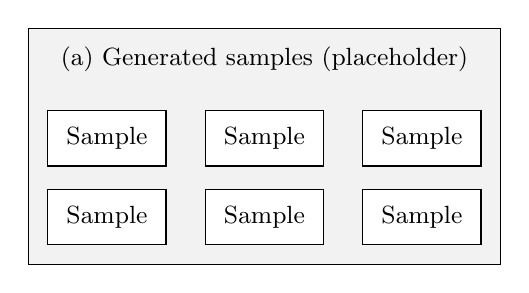
\begin{tikzpicture}[scale=1]
\draw[fill=gray!10] (0,0) rectangle (6,3);
\foreach \x in {0,1,2} \foreach \y in {0,1} {
  \draw[fill=white] (0.25+2*\x,0.25+1.0*\y) rectangle (1.75+2*\x,0.95+1.0*\y);
  \node at (1+2*\x,0.6+1.0*\y) {\small Sample};
}
\node at (3,2.6) {\small (a) Generated samples (placeholder)};
\end{tikzpicture}
\caption{}
\end{subfigure}
\hfill
\begin{subfigure}[b]{0.48\textwidth}
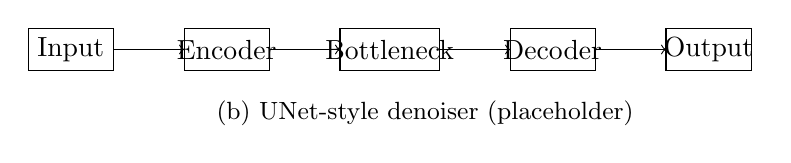
\begin{tikzpicture}[scale=0.9]
\draw (0,0) rectangle (1.2,0.6) node[midway]{Input};
\draw[->] (1.2,0.3) -- (2.2,0.3);
\draw (2.2,0) rectangle (3.4,0.6) node[midway]{Encoder};
\draw[->] (3.4,0.3) -- (4.4,0.3);
\draw (4.4,0) rectangle (5.8,0.6) node[midway]{Bottleneck};
\draw[->] (5.8,0.3) -- (6.8,0.3);
\draw (6.8,0) rectangle (8.0,0.6) node[midway]{Decoder};
\draw[->] (8.0,0.3) -- (9.0,0.3);
\draw (9.0,0) rectangle (10.2,0.6) node[midway]{Output};
\node at (5.6,-0.6) {\small (b) UNet-style denoiser (placeholder)};
\end{tikzpicture}
\caption{}
\end{subfigure}
\caption{Qualitative placeholders: (a) sample grid, (b) model architecture.}
\label{fig:samples}
\end{figure}

\section{Discussion and Conclusion}
Our synthetic results suggest that conditioning via FiLM-style modulation substantially improves sample quality compared to naive conditioning, consistent with prior findings~\cite{rombach2022high}. Future work could explore classifier-free guidance~\cite{ho2022classifierfree} and faster sampling methods~\cite{song2021score}.


\bibliographystyle{plain}
\bibliography{ref}

\end{document}
